%!TEX root = ../../master.tex


\begin{theorem}
    Visualization and tangibility are important in conveying cloud computing concepts to accomodate engineering students' learning style preferences. In order to align the students' mental model with the real world, a tangible cloud computing cluster needs to be designed and implemented as a mediating object.
\end{theorem}

\noindent
The previous three chapters introduced many cloud computing concepts. In order to teach and convey these concepts, we introduce a small-scale cloud computing cluster, KubeCloud, as a mediating learning object. The focus of this chapter is the process of specifying, designing, and implementing KubeCloud (Figure~\ref{fig:raspberry_pi_cluster}).

\begin{figure}[H]
    \centering
    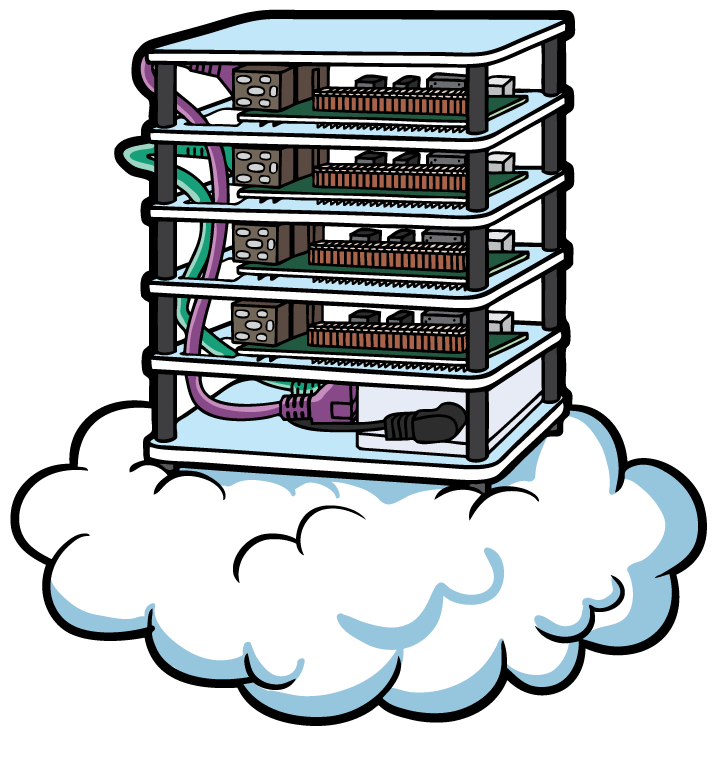
\includegraphics[width=6cm]{figures/raspberry_pi_cluster}
    \caption{Tangible Cloud Computing Cluster}
    \label{fig:raspberry_pi_cluster}
\end{figure}

\noindent
KubeCloud is designed to accommodate the learning style preferences identified by Felder and Silverman (Section~\ref{section:learning_styles}): sensory, visual, active, and sequential. These learning style preferences confirm the need for a learning object. Our experiment, presented later, confirmed three out of four of these preferred learning styles for the students participating in the course presented in this master's thesis. To accommodate the students' preferences and to create an active, sensory learning environment, KubeCloud shall be able to visualize and present concepts and allow for practical hands-on group work to foster social interaction and experimentation. In agreement with Churchill's classification of learning objects, KubeCloud shall be used as a: Presentation object, Practice object, Simulation object, and Conceptual object.
KubeCloud has to be a practice object to foster learning by doing. The workshop format involves the use of KubeCloud as a practice object. Presentations of concepts in cloud computing have to be demonstrated using KubeCloud. KubeCloud will, therefore, act as a presentation object. KubeCloud shall, furthermore, improve the students' skills of real life technologies, and must, therefore, act as a simulation object representing a small-scale real-life system. Lastly, KubeCloud further acts as a conceptual model e.g. by visualizing a small-scale data center.  